\documentclass[teaching.portfolio.tex]{subfiles}
\begin{document}
%\section{Math 017}
%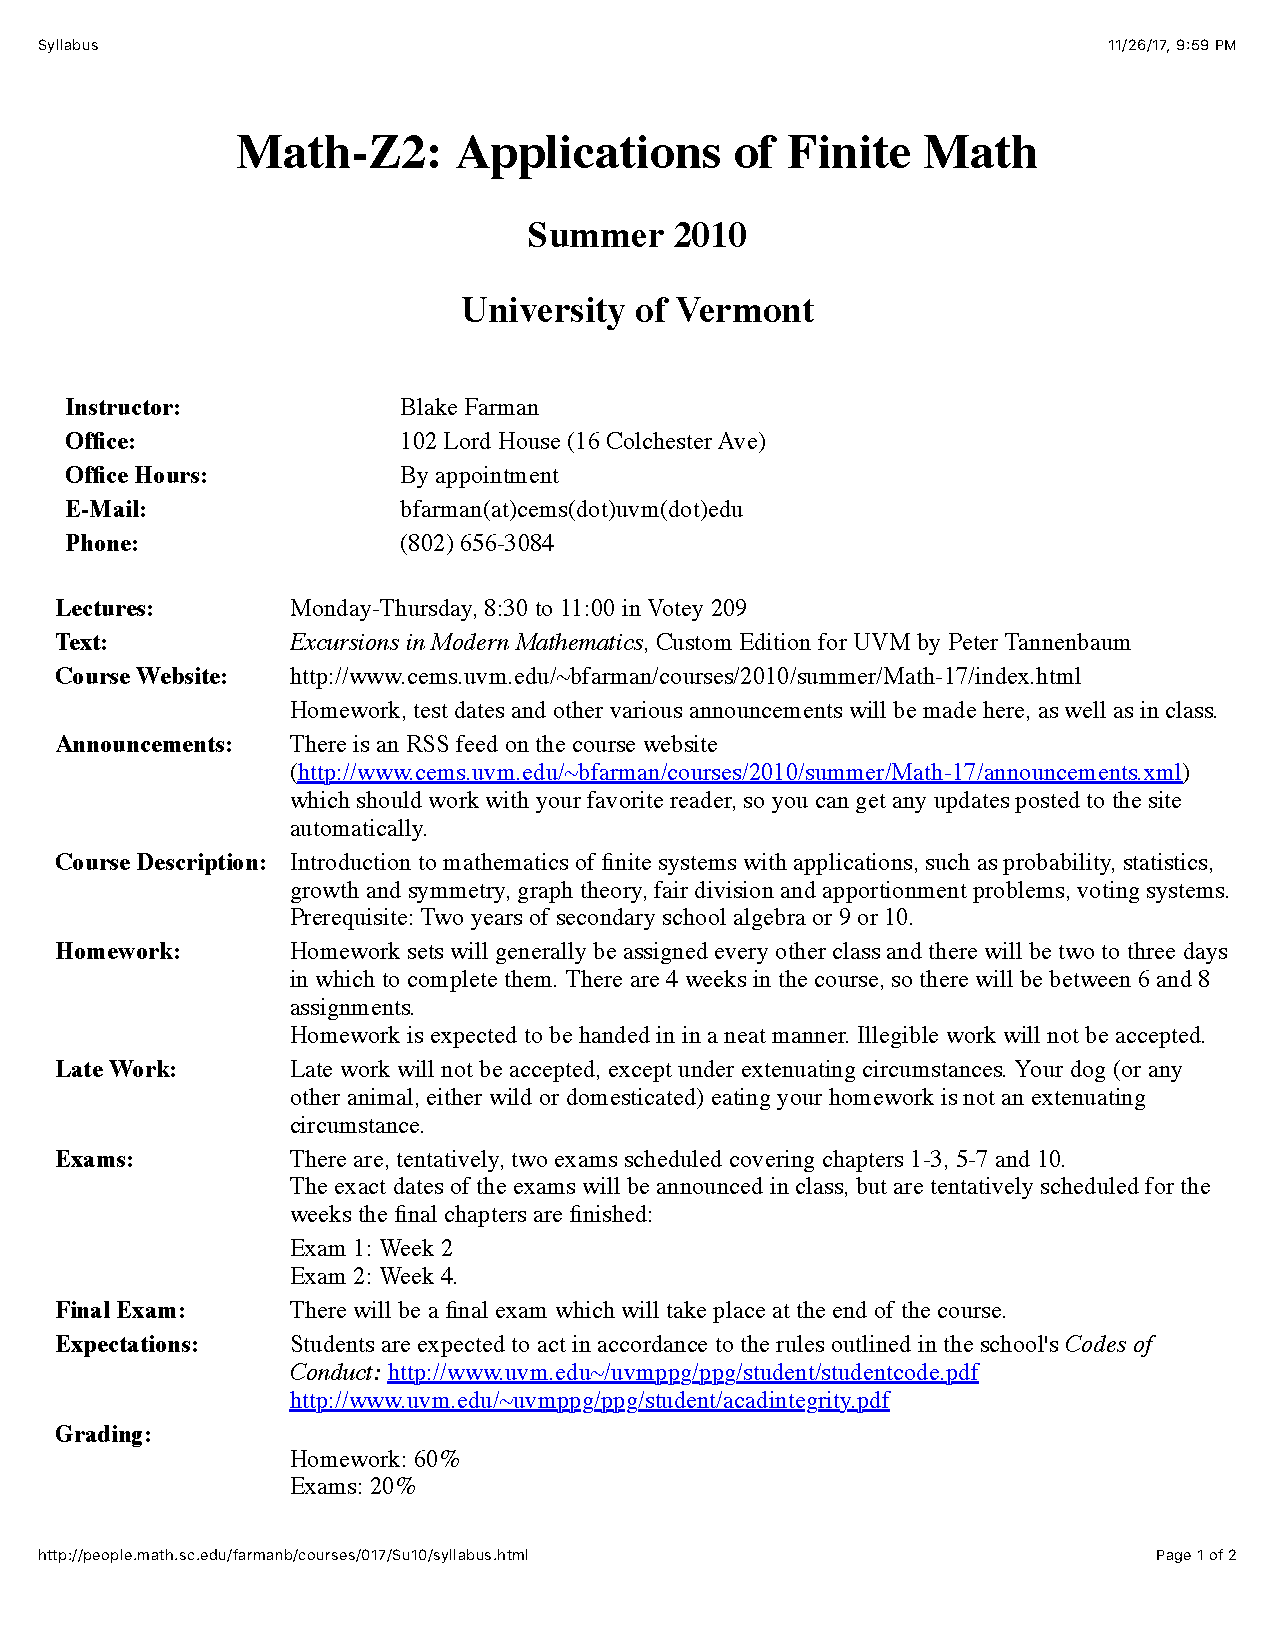
\includepdf[scale=0.8,pages=1,pagecommand=\subsection{Syllabus}]{../syllabi/syllabus-017.pdf}
%\includepdf[scale=0.8,pages=2-]{../syllabi/syllabus-017.pdf}
%\section{Math 019}
%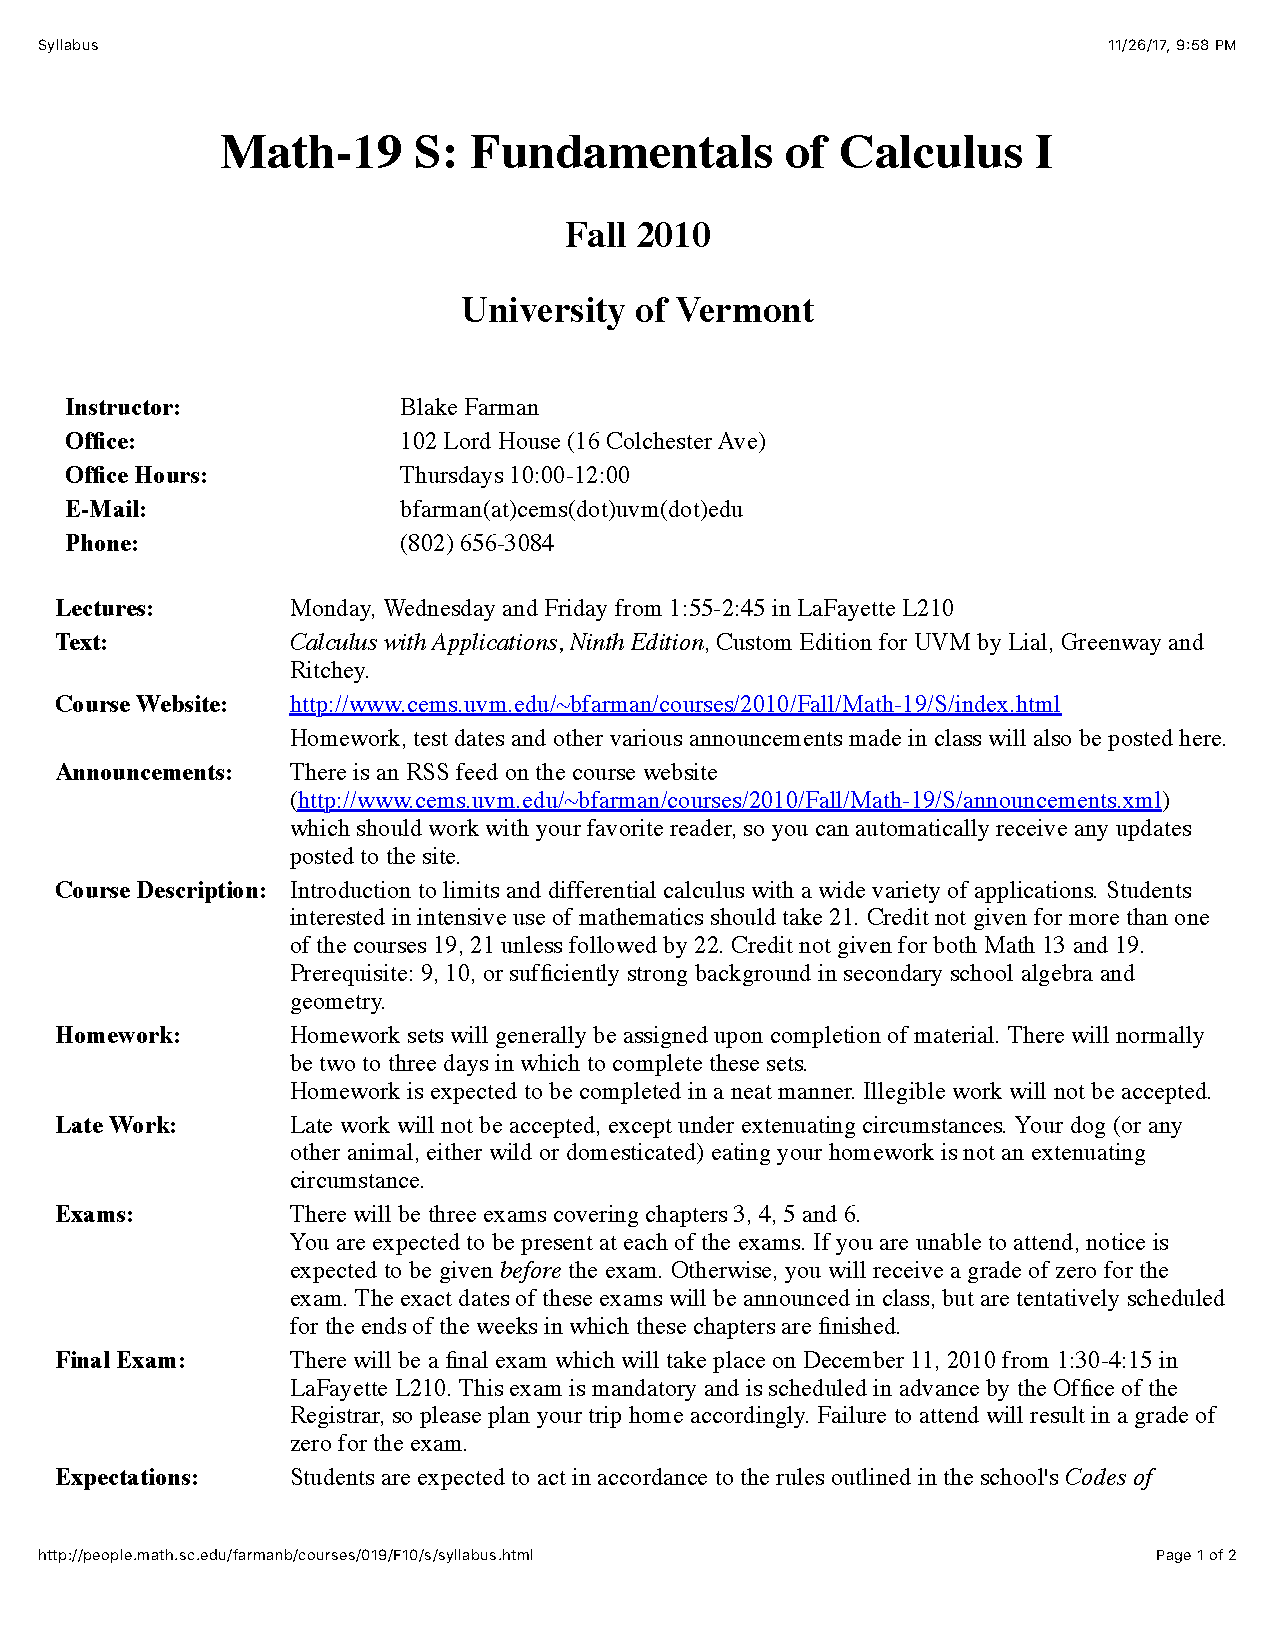
\includepdf[scale=0.8,pages=1,pagecommand=\subsection{Syllabus}]{../syllabi/syllabus-019.pdf}
%\includepdf[scale=0.8,pages=2-]{../syllabi/syllabus-019.pdf}
%\section{Math 111}
%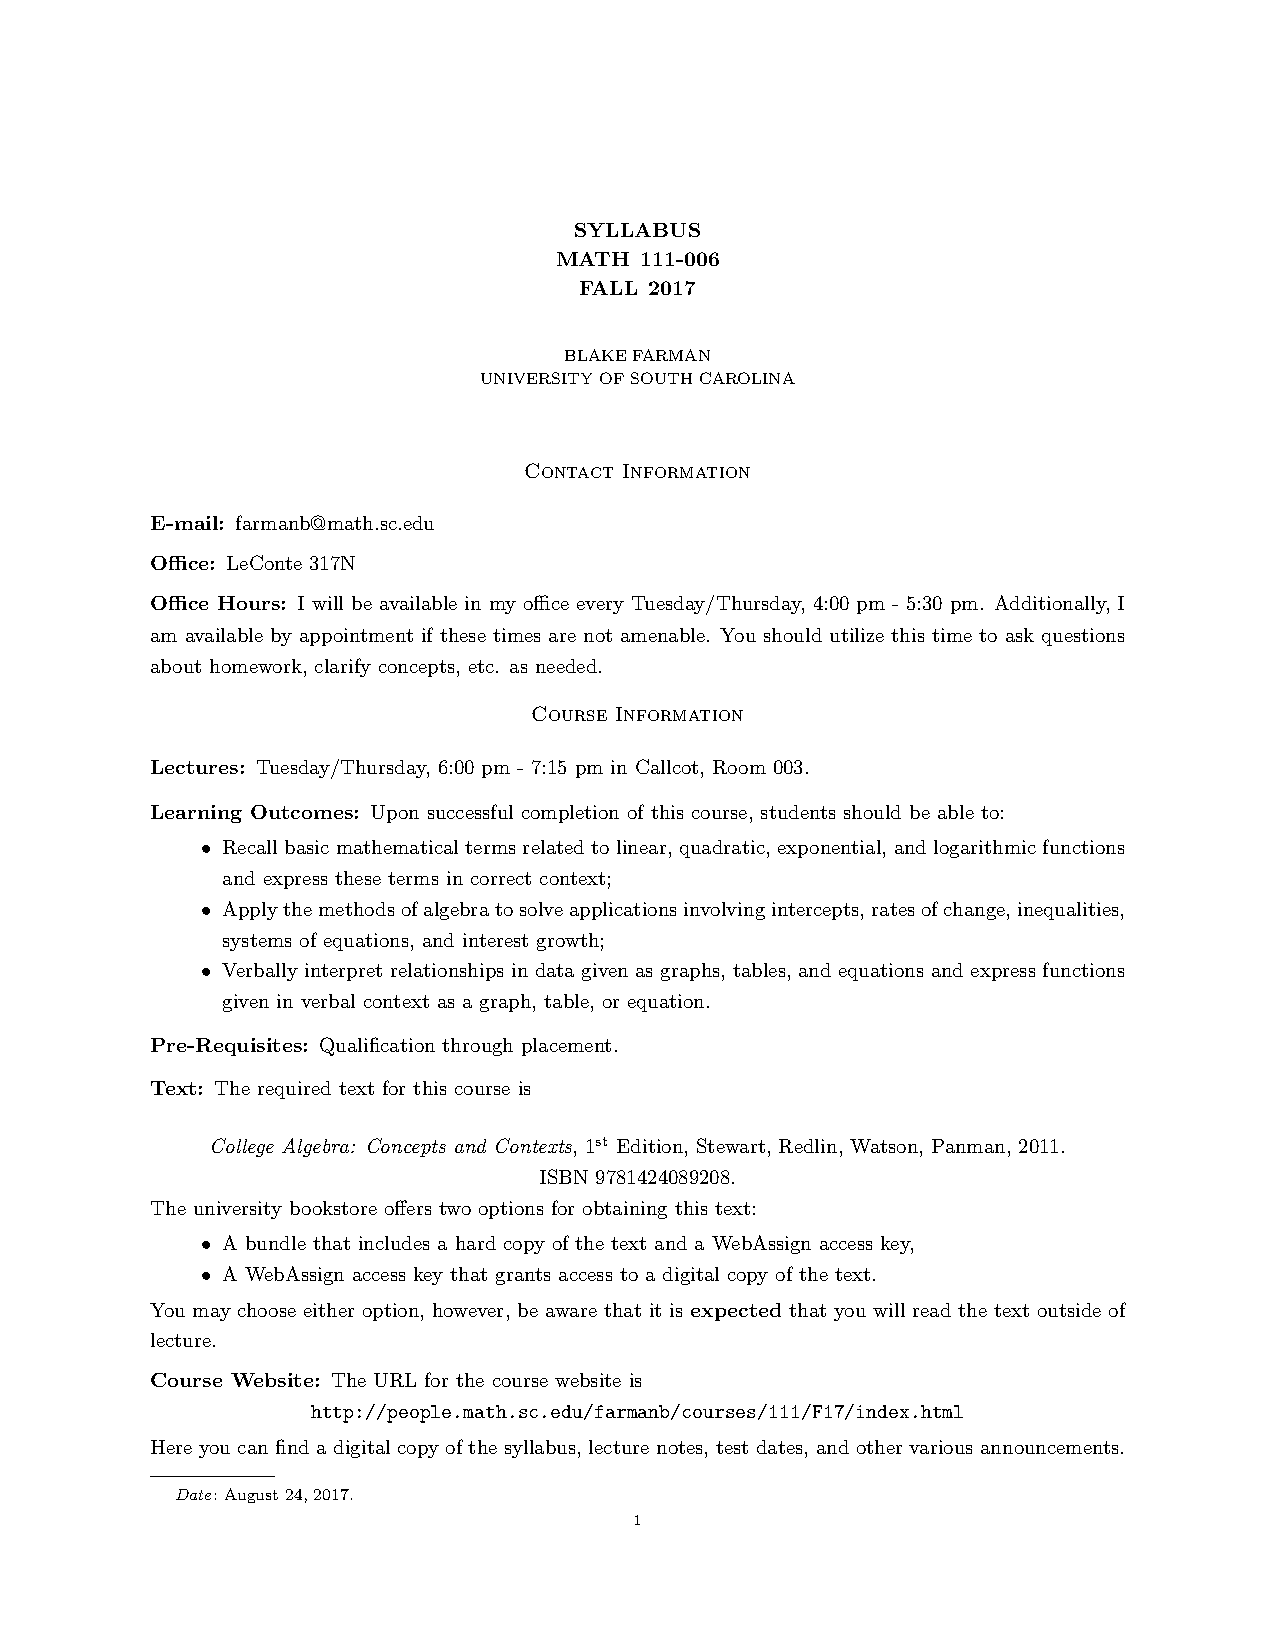
\includepdf[scale=0.8,pages=1,pagecommand=\subsection{Syllabus}]{../syllabi/syllabus-111-006.pdf}
%\includepdf[scale=0.8,pages=2-]{../syllabi/syllabus-111-006.pdf}
%\section{Math 115}
%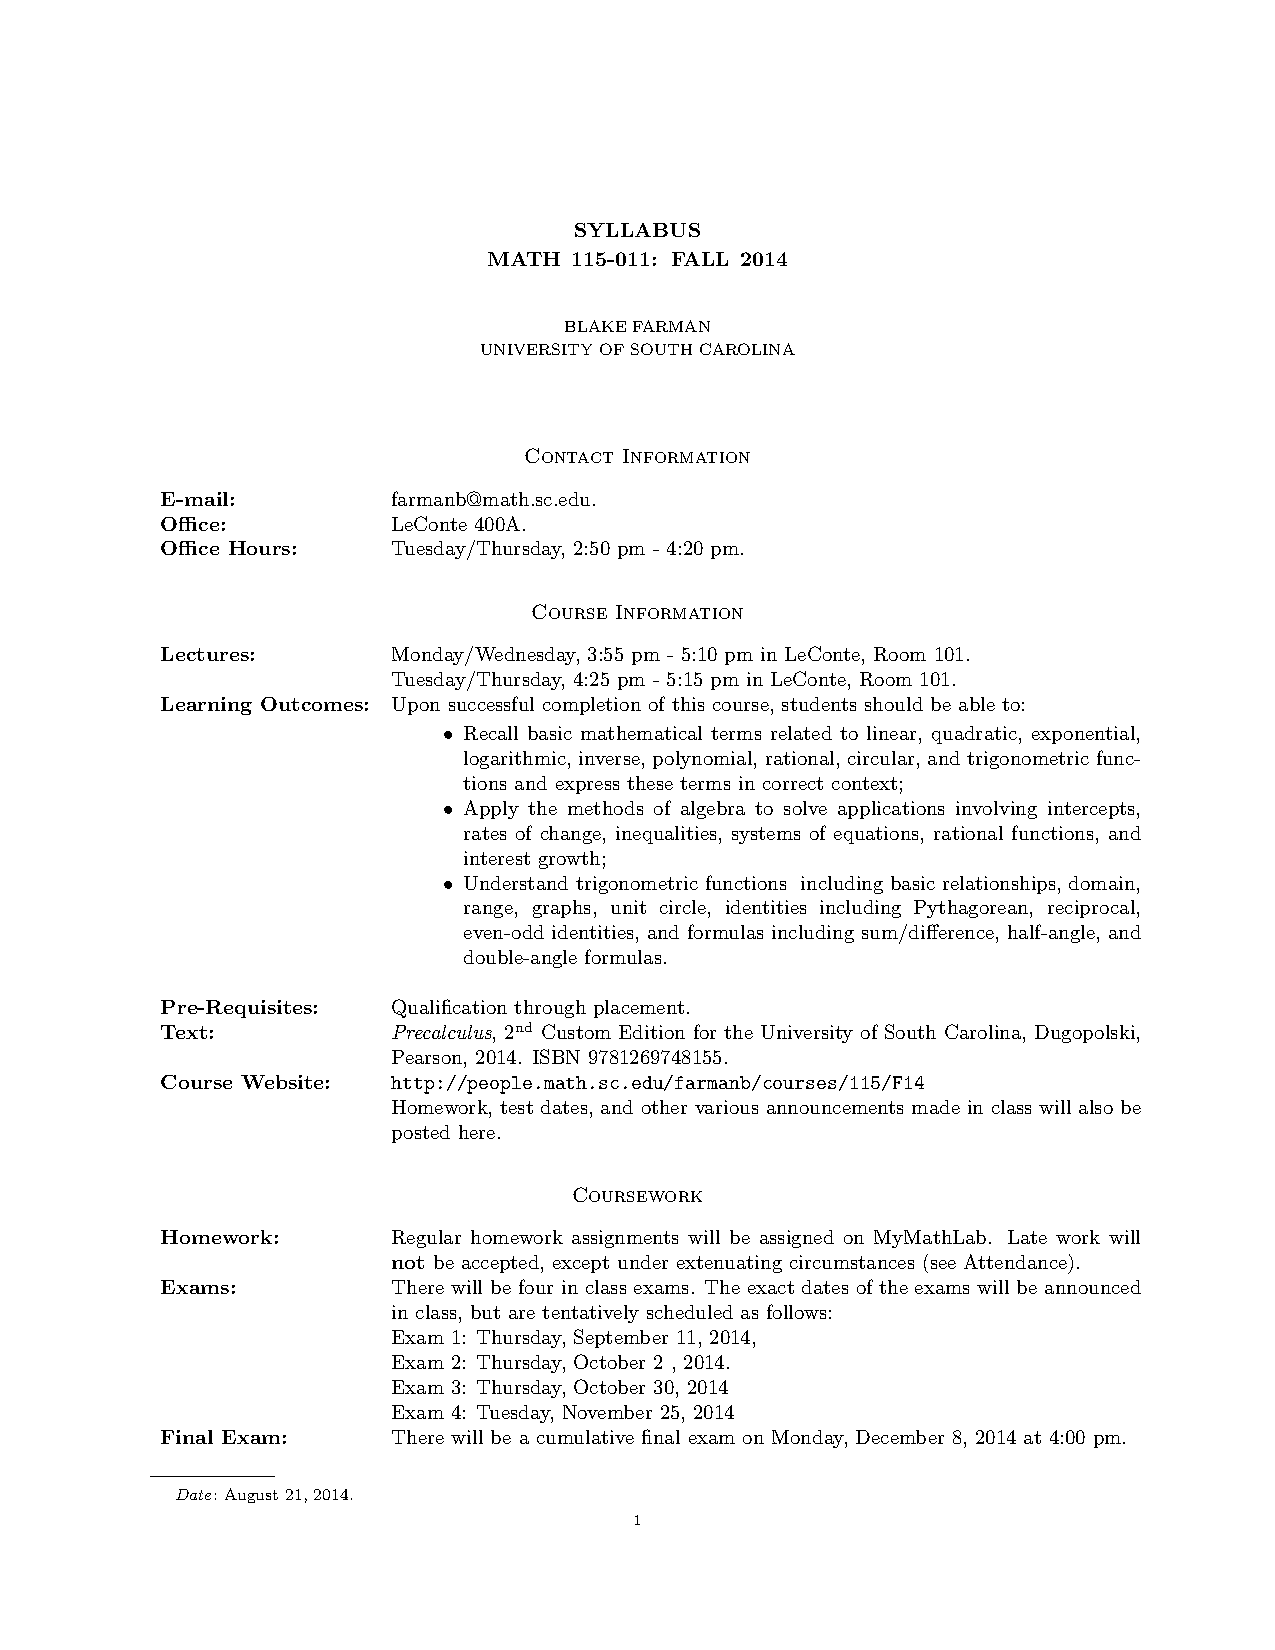
\includepdf[scale=0.8,pages=1,pagecommand=\subsection{Syllabus}]{../syllabi/syllabus-115-011.pdf}
%\includepdf[scale=0.8,pages=2-]{../syllabi/syllabus-115-011.pdf}
%\section{Math 116}
%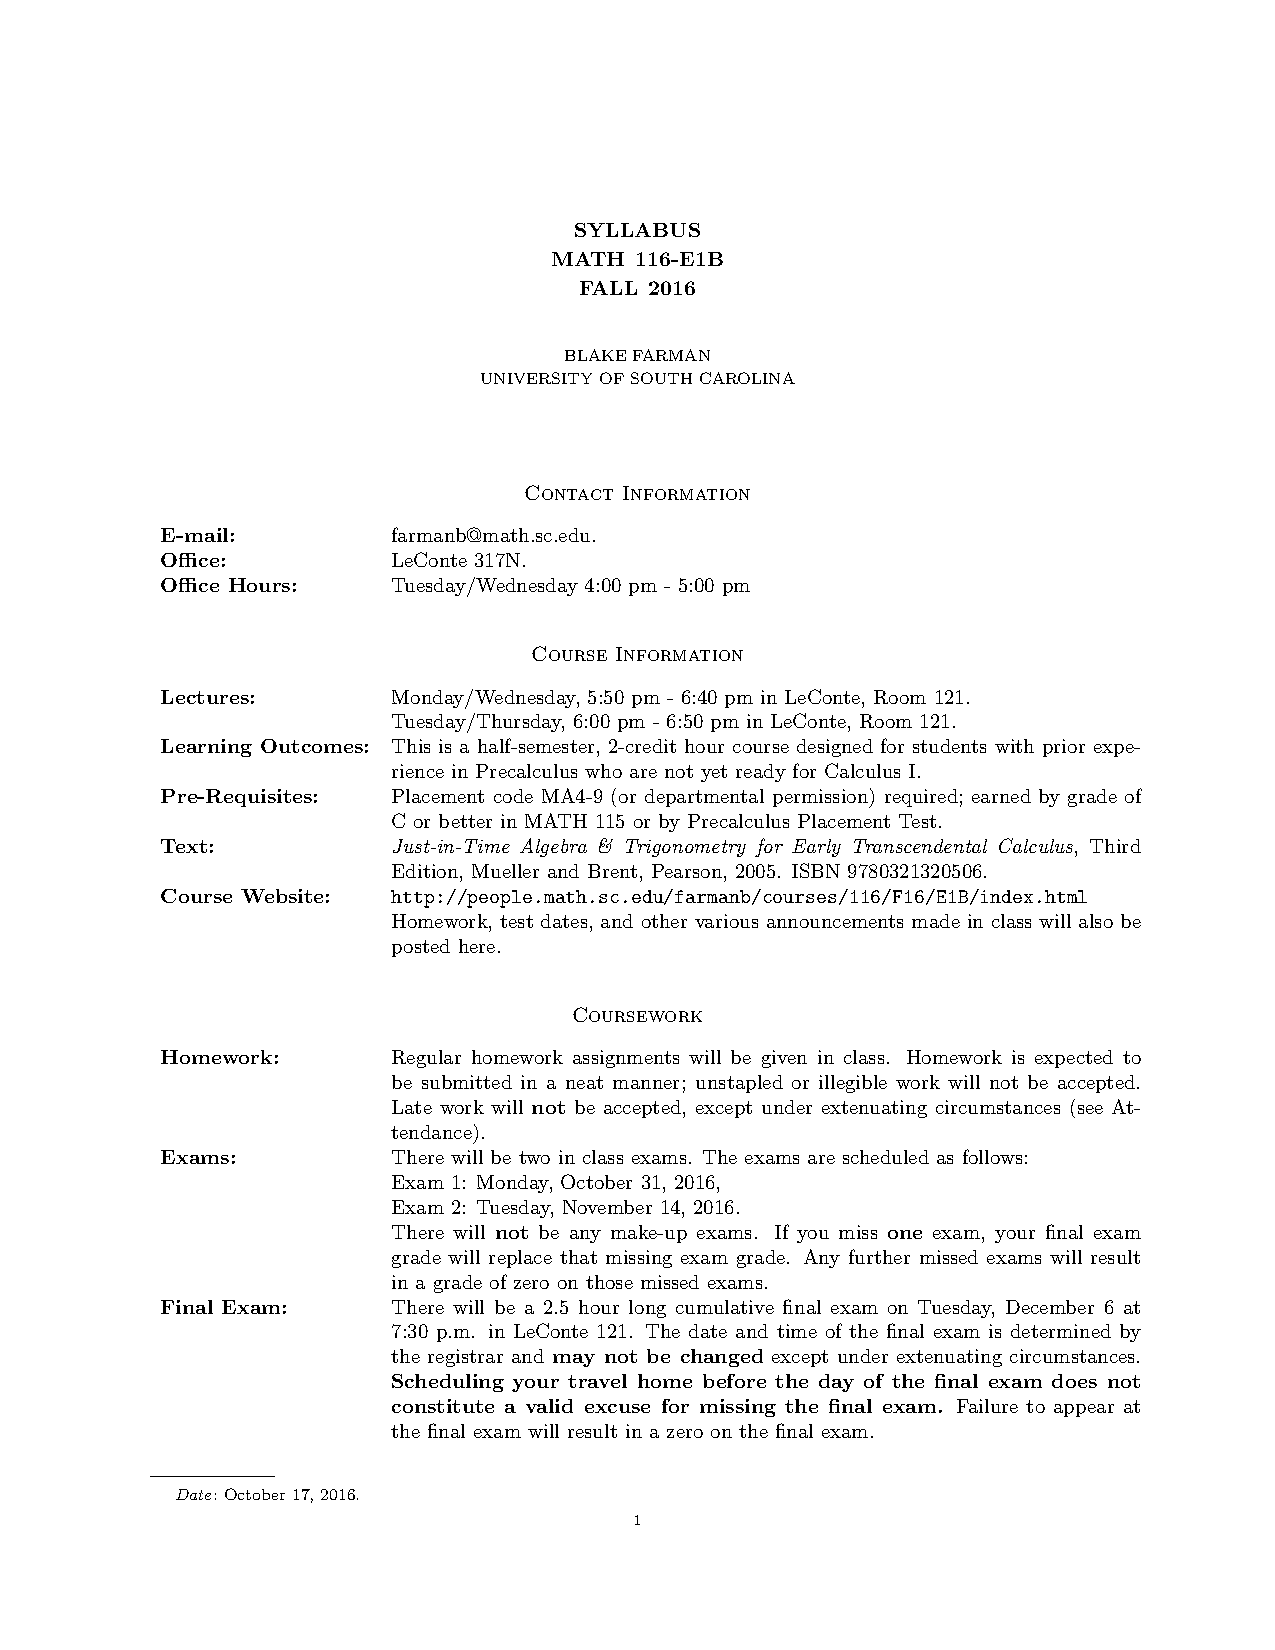
\includepdf[scale=0.8,pages=1,pagecommand=\subsection{Syllabus}]{../syllabi/syllabus-116-E1B.pdf}
%\includepdf[scale=0.8,pages=2-]{../syllabi/syllabus-116-E1B.pdf}
%\section{Math 122}
%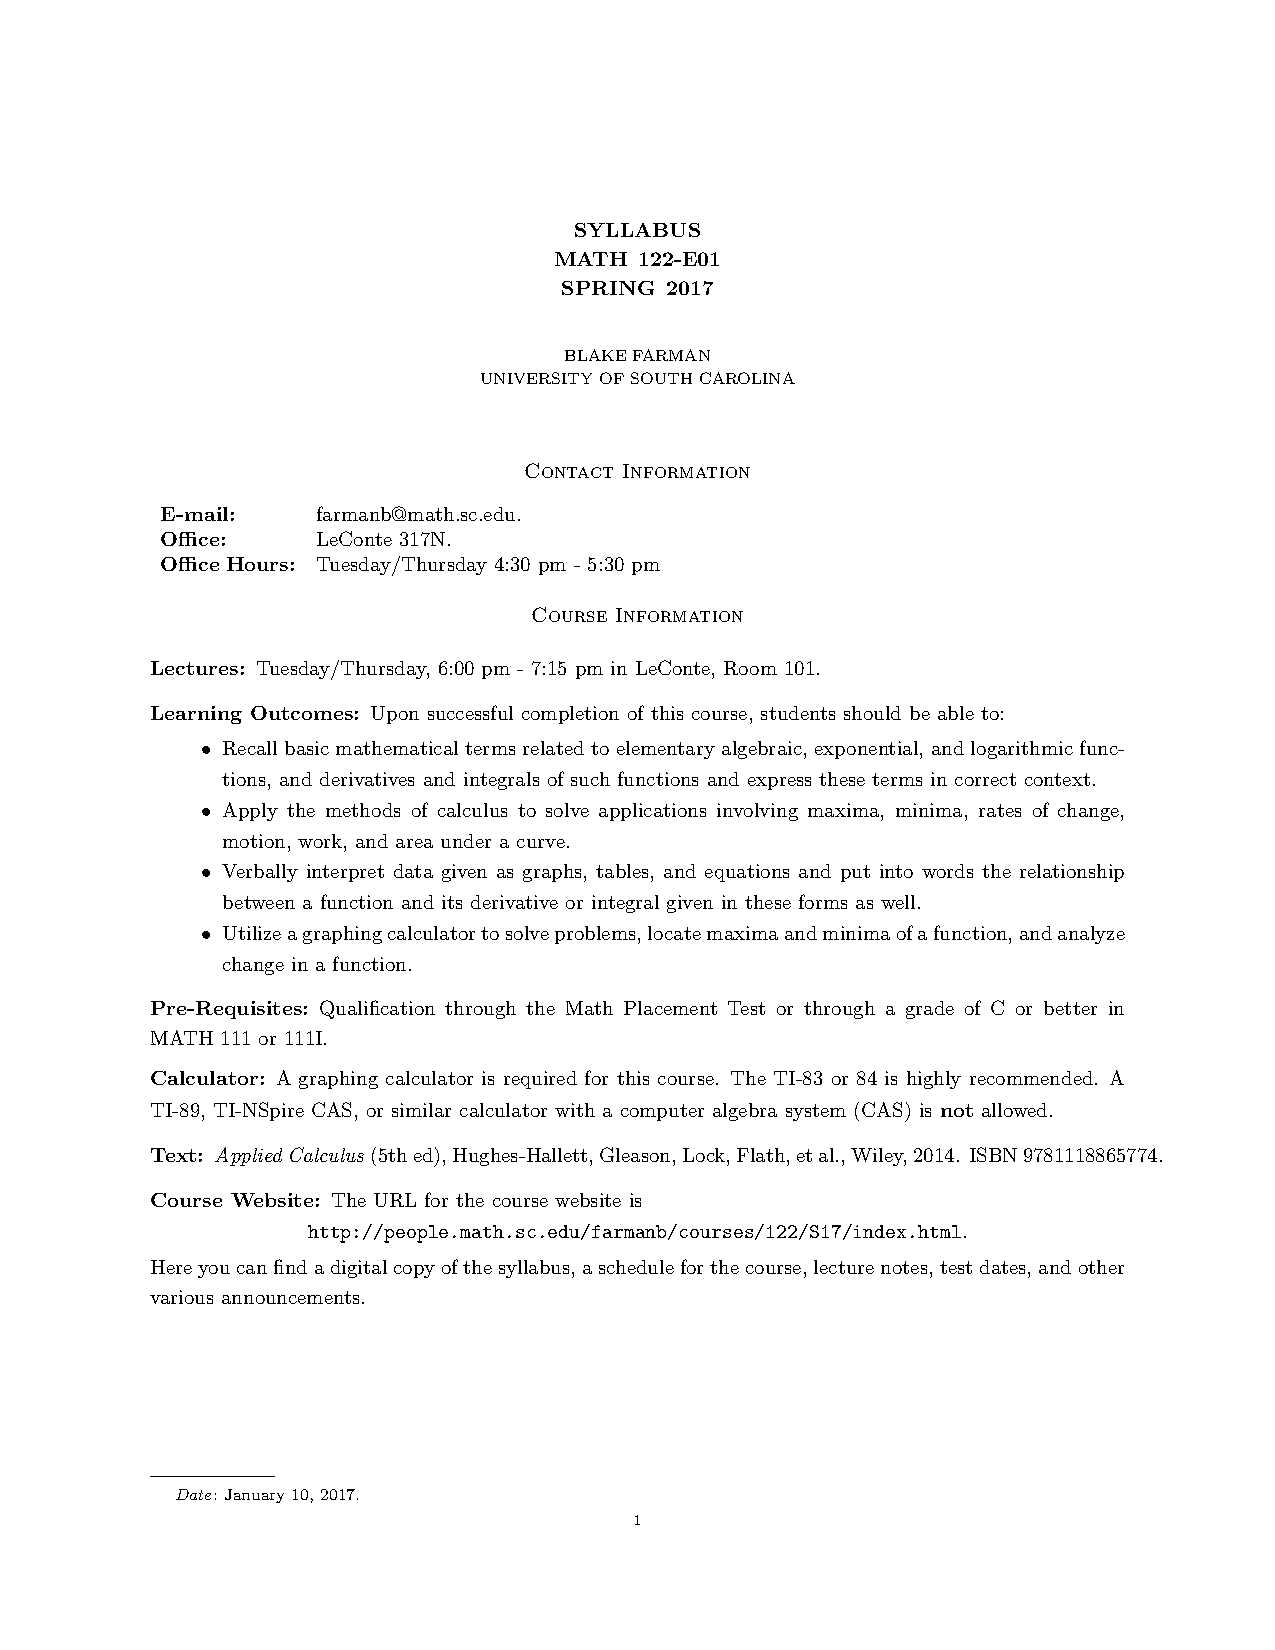
\includepdf[scale=0.8,pages=1,pagecommand=\section{Sample Syllabus}]{../syllabi/syllabus-122-E01.pdf}
%\includepdf[scale=0.8,pages=2-]{../syllabi/syllabus-122-E01.pdf}
%\section{Math 142}
%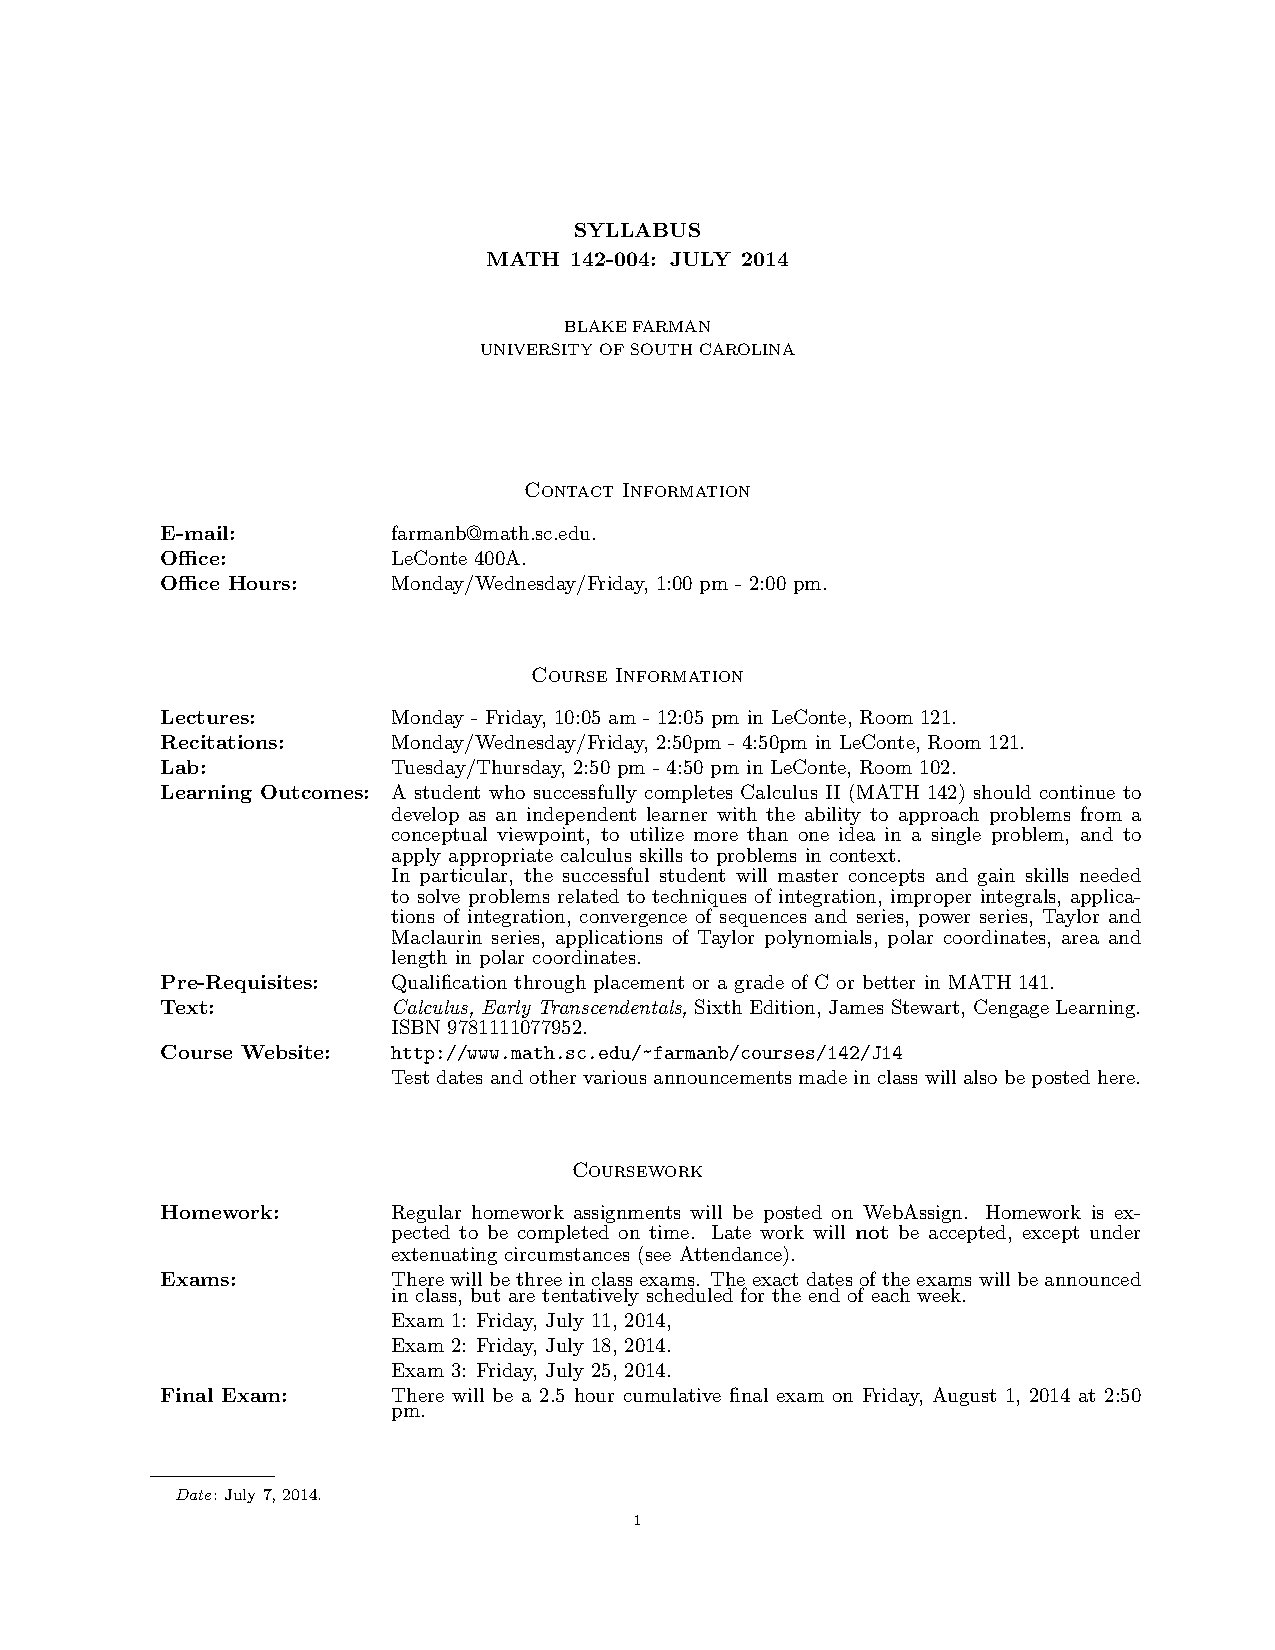
\includepdf[scale=0.8,pages=1,pagecommand=\subsection{Syllabus}]{../syllabi/syllabus-142-004.pdf}
%\includepdf[scale=0.8,pages=2-]{../syllabi/syllabus-142-004.pdf}
%\section{Math 170}
%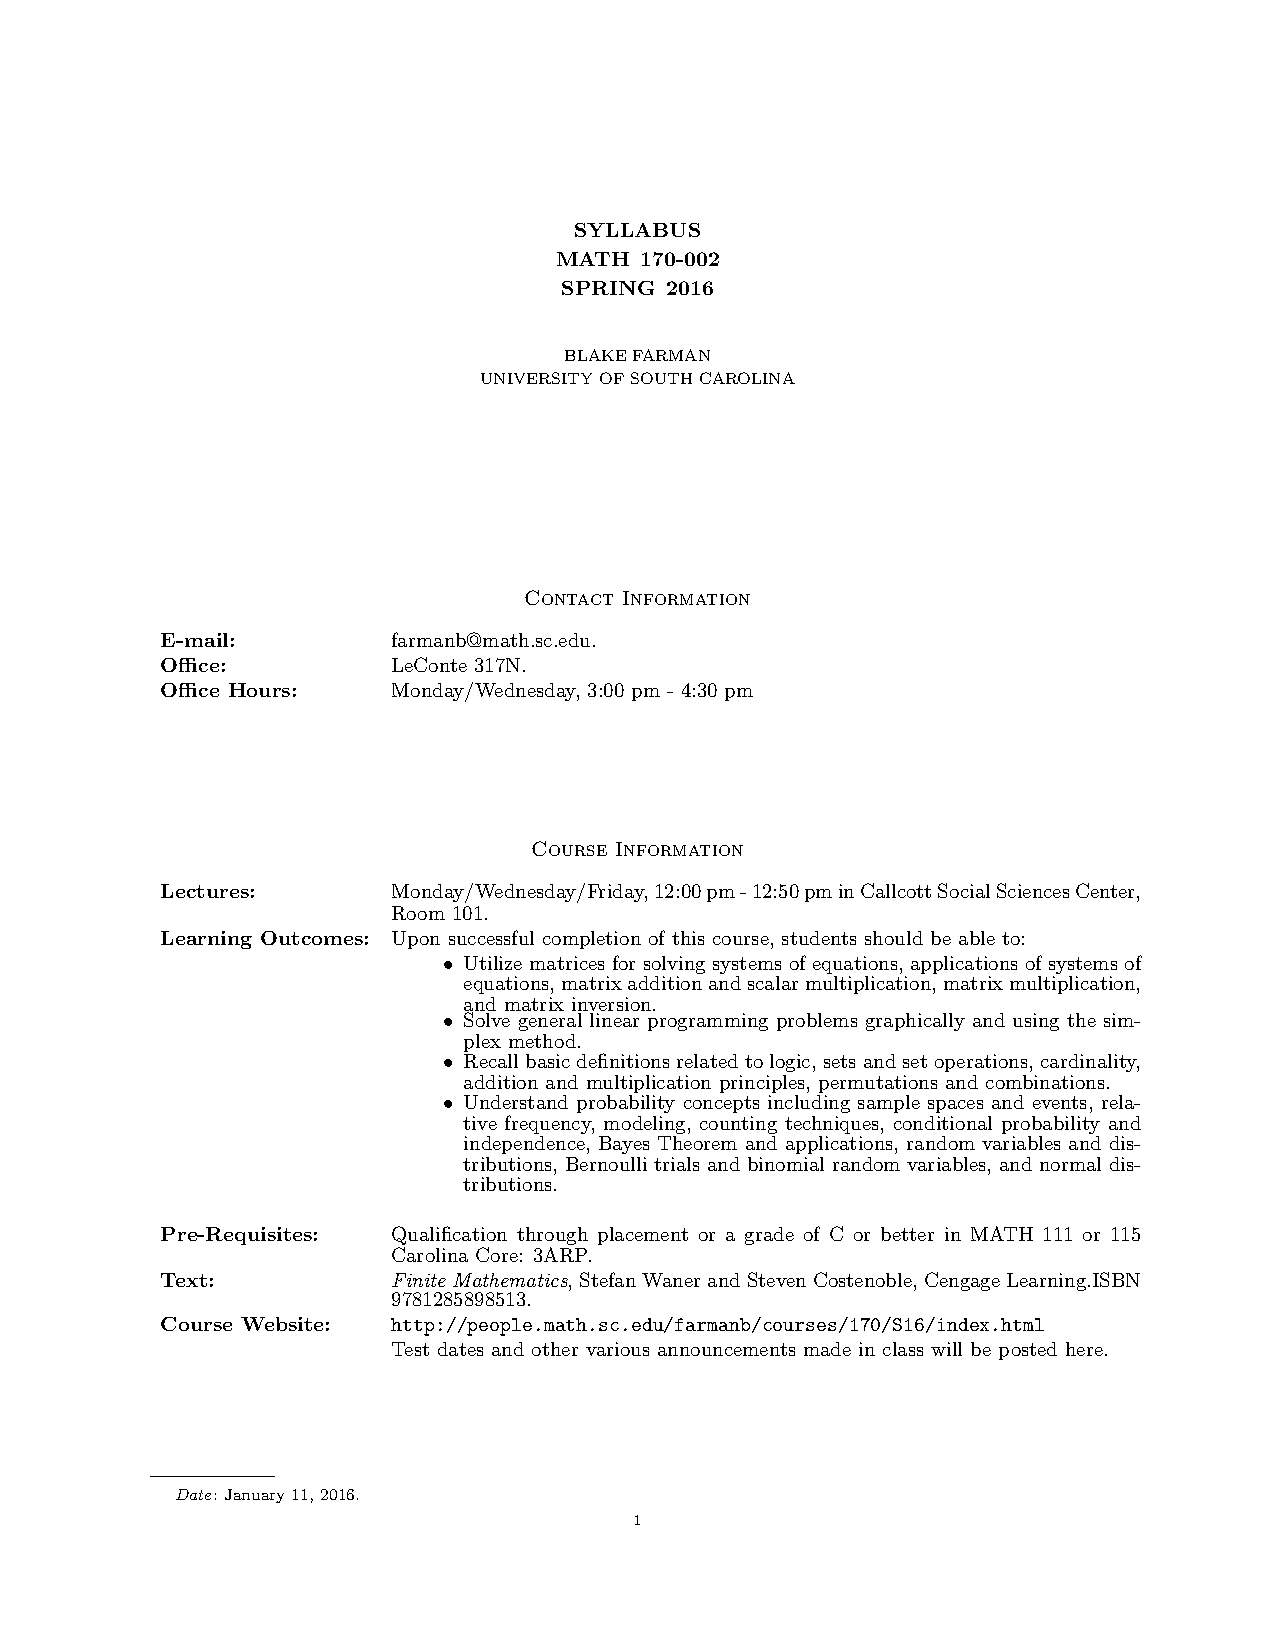
\includepdf[scale=0.8,pages=1,pagecommand=\subsection{Syllabus}]{../syllabi/syllabus-170-002.pdf}
%\includepdf[scale=0.8,pages=2-]{../syllabi/syllabus-170-002.pdf}

\subsection{Sample Syllabus}\hfill\\
\noindent
\textbf{Contact Information}\\
\noindent
\begin{tabular}{p{.9in}p{5in}}
  \textbf{E-mail:} &\href{mailto:farmanb@math.sc.edu}{farmanb@math.sc.edu}.\\
  \textbf{Office:} & LeConte 317N.\\
  \textbf{Office Hours:} & Tuesday/Thursday 4:30 pm - 5:30 pm
\end{tabular}

\begin{center}
  \textsc{Course Information}
\end{center}
\noindent
\textbf{Lectures:}
Tuesday/Thursday,  6:00 pm - 7:15 pm in LeConte, Room 101.\\
\textbf{Learning Outcomes:} 
Upon successful completion of this course, students should be able to:
\begin{itemize}
\item
  Recall basic mathematical terms related to elementary algebraic, exponential, and logarithmic functions, and derivatives and integrals of such functions and express these terms in correct context.
\item
  Apply the methods of calculus to solve applications involving maxima, minima, rates of change, motion, work, and area under a curve.
\item
  Verbally interpret data given as graphs, tables, and equations and put into words the relationship between a function and its derivative or integral given in these forms as well.
\item
  Utilize a graphing calculator to solve problems, locate maxima and minima of a function, and analyze change in a function.
\end{itemize}

\noindent
\textbf{Pre-Requisites:} 
Qualification through the Math Placement Test or through a grade of C or better in MATH 111 or 111I.\\

\noindent
\textbf{Calculator:}
A graphing calculator is required for this course.
The TI-83 or 84 is highly recommended.
A TI-89, TI-NSpire CAS, or similar calculator with a computer algebra system (CAS) is \textbf{not} allowed.\\

\noindent
\textbf{Text:} 
\textit{Applied Calculus} (5th ed), Hughes-Hallett, Gleason, Lock, Flath, et al., Wiley, 2014.  ISBN 9781118865774.\\

\noindent
\textbf{Course Website:} 
The URL for the course website is
\begin{center}
  \url{http://people.math.sc.edu/farmanb/courses/122/S17/index.html}.
\end{center}
Here you can find a digital copy of the syllabus, a schedule for the course, lecture notes, test dates, and other various announcements.

\noindent
\begin{center}
  \textsc{Coursework}
\end{center}

\noindent
\textbf{Homework:} 
Homework assignments will be made available through Wiley Plus.
The course is located at
\begin{center}
  \url{http://www.wileyplus.com/class/557219}.
\end{center}
Homework is expected to be submitted on time.
Late work will \textbf{not} be accepted.\\

\noindent
\textbf{Exams:} 
There will be three in class exams.
The exams are \textbf{tentatively} scheduled as follows:
\begin{center}
  \begin{tabular}{ll}
    Exam 1: & Tuesday, February 7, 2017,\\
    Exam 2: & Thursday, March 16, 2017,\\
    Exam 3: & Thursday, April 13, 2017.
  \end{tabular}
\end{center}
\noindent
There will \textbf{not} be any make-up exams.
If you miss \textbf{one} exam, your final exam grade will replace that missing exam grade.
Any further missed exams will result in a grade of zero on those missed exams.
\textbf{This policy is intended only for exams missed due to illness, accidents, etc.  
  It does NOT mean that your lowest exam grade will be dropped.}\\

\noindent
\textbf{Final Exam:} 
There will be a 2.5 hour long cumulative final exam on Thursday, April 27 at 7:30 p.m. in LeConte 101.
The date and time of the final exam is determined by the registrar and \textbf{may not be changed} except under extreme circumstances.
\textbf{Scheduling your travel home before the day of the final exam does not constitute a valid excuse for rescheduling the final exam.}
Failure to appear at the final exam will result in a zero on the final exam.

\begin{center}
  \textsc{Grading}
\end{center}

\noindent
\textbf{Scale:} 
Grades will be assigned on the following scale:
\begin{center}
  \begin{tabular}{ll}
    A: &90-100\%,\\
    B: & 80-89\%,\\
    C: & 70-79\%,\\
    D: & 60-69\%,\\
    F: & $<$ 60\%.\\
  \end{tabular}
\end{center}

\noindent
\textbf{Weights:} 
Final grades will be calculated with the following weights:
\begin{center}
  \begin{tabular}{lr}
    Homework: & 25\%,\\
    Exams: & 45\%,\\
    Final Exam: & 30\%.\\
  \end{tabular}
\end{center}

\begin{center}
  \textsc{Student Success Center}
\end{center}

\noindent
In partnership with UofSC faculty, the Student Success Center (SSC) offers a number of programs to assist you in better understanding your course material and to aid you on your path to success. 
SSC programs are facilitated by professional staff, graduate students, and trained undergraduate peer leaders who have previously excelled in their courses.
Resources available to students include: 
\begin{itemize}
\item 
  \textbf{Peer Tutoring:} make a one-on-one appointment with a Peer Tutor by going to \url{www.sc.edu/success}. 
  If a course is not on the semester’s supported-course list, there is a process for requesting assistance. 
  The full schedule of days/times/locations for drop-in and Online Tutoring hours can also be viewed on the SSC website.
\item
  \textbf{Supplemental Instruction (SI):} attend SI Sessions to focus on the most difficult content being covered in class. 
  SI Leaders are assigned to specific sections of courses and hold three weekly study sessions that can serve as “built-in study time.” 
  The schedule is posted on the SSC website each week and will also be communicated by the SI Leader.
\item
  \textbf{Peer Success Consultations:} make a one-on-one Success Consultation with a Peer Consultant to work on developing study skills, setting goals, and connecting to a variety of campus resources. 
  Your instructor may communicate with the SSC via Success Connect, an online referral system, regarding your progress in the course. 
  If contacted by the SSC, please schedule a Success Consultation. 
  Success Connect referrals are not punitive and any information shared by your professor is confidential and subject to FERPA regulations.
\end{itemize}
SSC services are offered to all UofSC undergraduates at no additional cost.
You are invited to call the Student Success Hotline at (803) 777-1000, visit \url{www.sc.edu/success}, or come to the SSC in the Thomas Cooper Library (Mezzanine Level) to check schedules and make appointments. 

\begin{center}
  \textsc{Expectations}
\end{center}

\noindent
\textbf{Academic Integrity:} 
\textit{As a Carolinian...I will practice personal and academic integrity.}\\

\noindent 
The University of South Carolina expects high standards in all areas from its students.
The University, as well as the faculty, staff, alumni, and students believe strongly in the Honor Code.
This Code requires acceptance of certain responsibilities and agreement by all students to abide by the spirit of the Honor Code upon entering the University of South Carolina.
In order that you may better understand the required responsibilities, the general University community codes are outlined below.

\begin{enumerate}
\item
  It shall be the responsibility of every faculty member, student, administrator and staff member of the University community to uphold and maintain the academic standards and integrity of the University of South Carolina.
\item
  Any member of the University community, who has reasonable grounds to believe that an infraction of the Honor Code has occured, has an obligation to report the alleged violation.
  Violation of any of the following standards subjects the student to disciplinary action: improper collaboration, cheating, lying, bribery, and plagiarism.
\end{enumerate}

\noindent
Your enrollment in this class signifies your willingness to accept these responsibilities and uphold the Honor Code of the University of South Carolina.
Please review the Honor Code via
\begin{center}
  \url{https://www.sa.sc.edu/academicintegrity/}
\end{center}

\noindent
Any deviation from this expectation \textbf{will result in a grade of F in the course} and disciplinary action through the Office of Academic Integrity.\\

\noindent
\textbf{Attendance:} 
Students are obligated to complete all assigned work promptly, to attend class regularly, and to participate in whatever class discussion may occur.\\

\noindent
The following events or circumstances are potentially excusable absences:
\begin{itemize}
\item
  participation in an authorized University activity (such as musical performances, academic competitions, or varsity athletic events in which the student plays a formal role in a University sanctioned event),
\item
  required participation in military duties,
\item
  mandatory admission interviews for professional or graduate school which cannot be rescheduled,
\item
  participation in legal proceedings or administrative duties that require a student's presence,
\item
  death or major illness in a student’s immediate family,
\item
  illness of a dependent family member
\item
  religious holy day if listed on \url{www.interfaithcalendar.org},
\item
  illness that is too severe or contagious for the student to attend class,
\item
  weather-related emergencies.
\end{itemize}
For more information, see the University Attendance Policy:
\begin{center}
  \url{http://bulletin.sc.edu/index.php?catoid=56}.
\end{center}

\subsection{Sample Exam}
The following is an exam given to my Calculus II class in July 2014.
\begin{thm}
  Find the volume of the solid obtained by rotating the region bounded by the curves $f(x) = 4(x - 2)^2$ and $g(x) = x^2 - 4x + 7$ about the $y$-axis.
\end{thm}

\textbf{Integration}\\

\noindent For each of the following problems, decide which method of integration is appropriate and compute the given integrals.
You will find some useful trigonmetric identities on the last page.
If you need more space for a problem, use the back of the page.

\begin{thm}
  Compute $\displaystyle{\int\sin^3(\theta)\cos^2(\theta)d\theta}$.
\end{thm}

\begin{thm}
  Compute $\displaystyle{\int \frac{\ln(x)}{x^2}dx}$.
\end{thm}

\begin{thm}
  Compute $\displaystyle{\int\frac{dx}{x^2\sqrt{x^2-9}}}$.
\end{thm}

\begin{thm}
  Compute $\displaystyle{\int\frac{x}{x^2 - 5x + 6}}dx$.
\end{thm}

\begin{thm}
  Explain why $\displaystyle{\int_0^3 \frac{dx}{\sqrt{x}}}$ is an improper integral, then evaluate it.
\end{thm}

\textbf{Series and Sequences}
\begin{thm}
  Express $5.\overline{5} = 5.55555\ldots$ as a rational number. [Hint: Geometric Series.]
\end{thm}

\noindent
Test the following series for convergence.
You may use any of the tests we covered in class, however you {\bf must indicate which test you use}.
\begin{thm}
  $\displaystyle{\sum_{k=1}^\infty \frac{2^k k!}{(k+2)!}}.$
\end{thm}

\begin{thm}
  $\displaystyle{\sum_{n=1}^\infty \frac{2^{2n}}{n^n}}$
\end{thm}

\textbf{Power Series}

\begin{thm}
  Find the Taylor expansion of $\ln(x)$ about $a = 2$ and find the radius of convergence and the interval of convergence for the series you find.
\end{thm}

\textbf{Bonus}

\begin{thm}
  Sketch the curve with polar equation $\displaystyle{r = \sin^2(2\theta)}$.
\end{thm}

\subsection{Sample Course Evaluations}
\includepdf[scale=0.8,pages=2]{../evaluations/USC/2017/spring/122-E01.pdf}
\includepdf[scale=0.8,pages=3-5]{../evaluations/USC/2017/spring/122-E01.pdf}
\includepdf[scale=0.8,pages=7-9]{../evaluations/USC/2017/spring/122-E01.pdf}
\includepdf[scale=0.8,pages=10-]{../evaluations/USC/2017/spring/122-E01.pdf}
\end{document}

